\documentclass[9pt,a4paper]{extarticle}
\usepackage[T1]{fontenc}
\usepackage{mathptmx}
\usepackage[scaled=0.82]{beramono}
\usepackage[a4paper,left=1.5cm,right=1.5cm,top=1.3cm,bottom=1.3cm]{geometry}
\usepackage{booktabs,tabularx,array,enumitem,titlesec,microtype,amssymb}
\usepackage{graphicx}
\usepackage{tikz}
\usetikzlibrary{arrows.meta,positioning}
\pagestyle{empty}
\setlength{\parindent}{0pt}
\setlength{\parskip}{4pt}
\titleformat{\section}{\large\bfseries}{\thesection}{0.6em}{}
\titlespacing*{\section}{0pt}{10pt}{3pt}
\setlist[itemize]{leftmargin=1.2em,itemsep=0pt,topsep=1pt,parsep=0pt}
\renewcommand{\arraystretch}{1.18}
\newcolumntype{L}{>{\raggedright\arraybackslash}X}
\newcommand{\code}[1]{{\small\texttt{#1}}}

\begin{document}
\textbf{Team No. 14}

\begin{center}
{\Large\bfseries Final Report}\\[2pt]
Qalam: Voice-Driven AI Incident Report Assistant (Qualcomm Problem Statement)\\
{\small Target device: Qualcomm QIDK (Snapdragon 8 Elite, Hexagon NPU V79), fully on-device and offline \;$\cdot$\; 11th October}
\end{center}

\section{What We Built}
\textbf{Qalam} (``kalam'', pen; Q for Qualcomm) turns a spoken account of an incident into a structured, validated and searchable report, entirely on the QIDK. The user taps one button, or says ``Hey Qalam'', and describes what happened in English or Hinglish. Whisper transcribes the speech on the device. \textbf{Qwen3-4B runs on the Hexagon NPU inside the app} and returns one function call that fills the form. A deterministic layer checks every value against what was actually said, a rule-based validator finds the mandatory fields still missing for that incident type, and the app asks only for those, by voice. The user reviews, submits, and the report lands in an on-device dashboard with search, hotspots and a conversational ``Ask'' tab. The app has \textbf{no internet permission}; an on-screen proof line shows the model, its live speed and ``0 B sent''.

\begin{center}\small
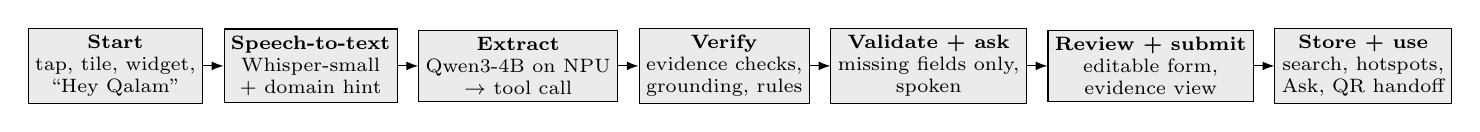
\begin{tikzpicture}[node distance=2.6mm,
  box/.style={draw,align=center,font=\scriptsize,inner sep=2.5pt,minimum height=9mm,fill=black!8}]
\node[box] (a) {\textbf{Start}\\tap, tile, widget,\\``Hey Qalam''};
\node[box,right=of a] (b) {\textbf{Speech-to-text}\\Whisper-small\\+ domain hint};
\node[box,right=of b] (c) {\textbf{Extract}\\Qwen3-4B on NPU\\$\rightarrow$ tool call};
\node[box,right=of c] (d) {\textbf{Verify}\\evidence checks,\\grounding, rules};
\node[box,right=of d] (e) {\textbf{Validate + ask}\\missing fields only,\\spoken};
\node[box,right=of e] (f) {\textbf{Review + submit}\\editable form,\\evidence view};
\node[box,right=of f] (g) {\textbf{Store + use}\\search, hotspots,\\Ask, QR handoff};
\foreach \x/\y in {a/b,b/c,c/d,d/e,e/f,f/g} \draw[-{Latex[length=1.5mm]}] (\x) -- (\y);
\end{tikzpicture}\\[1pt]
{\scriptsize Every stage is built and runs on the QIDK. Emergency wording short-circuits the loop: banner, response clock and ``Call ERT'' appear at once.}
\end{center}

\section{How It Works}
\begin{tabularx}{\linewidth}{@{}p{2.7cm}L@{}}
\toprule
\textbf{Component} & \textbf{Design and reasoning}\\
\midrule
Speech-to-text & Whisper-small (q5\_1, whisper.cpp, CPU) with Silero VAD end-pointing, noise suppression and peak normalisation. The app writes a short \emph{domain hint} (incident words, site place names) that biases the decoder; it fixed live mis-hearings such as ``water leak'' $\rightarrow$ ``virtual leap''.\\
LLM on the NPU & Qualcomm's pre-compiled \textbf{Qwen3-4B} Genie bundle (w4a16, 4096-token context, Apache-2.0) loaded in-app through JNI on the Hexagon V79. The chat template is selected by model family (Llama or Qwen), so a different bundle is a file swap, not a code change. Greedy decoding, thinking mode switched off, one NPU session at a time, 20\,s limit per call.\\
Function calling & The model only proposes \code{fill\_incident\_form} / \code{update\_incident\_fields}; the app parses, normalises and executes them. Output is taken as the first balanced JSON object, with one repair attempt.\\
The system layer (why the model cannot invent a report) & Deterministic checks between the model and the form: injuries, severity, place and time are kept only if the words support them; names and places are grounded in the transcript; a spoken self-correction (``at 10, no, 11'') is applied; life-at-risk wording forces CRITICAL; the keyword rules give the model a category hint and take over a turn if the model fails. Small talk (``hi, this is Ravi'') fills nothing: the app answers ``I didn't catch an incident. What happened?''.\\
Validator and follow-ups & Mandatory fields per incident type come from a taxonomy file, not from the model. The app asks for the missing ones only, at most two per question, in the reporter's own language (English or Hinglish), and stops after three rounds.\\
Emergency path & Critical wording raises a banner immediately and starts a \textbf{response clock}: elapsed time plus the site's immediate SOP steps as large tap targets, each logged with its time. In an emergency the app asks one question at most (where), then gets out of the way.\\
Robustness & Every failure has a defined behaviour: model error or timeout $\rightarrow$ rules engine answers that turn with a visible ``Fallback'' chip; silence $\rightarrow$ one spoken retry; unparseable output $\rightarrow$ repair, then manual fill. The draft is saved at every step.\\
Storage & Room/SQLite with full-text search, an audit log of every field change, the verbatim transcript and recording per turn, and an on-device vector index (MiniLM) for meaning-based search.\\
\bottomrule
\end{tabularx}

\textbf{Worked example, as it ran on the board (input from the problem statement)}

\begin{tabularx}{\linewidth}{@{}p{2.7cm}L@{}}
\toprule
User says & ``There was a water leak near Conference Room 2 around 10 AM. Maintenance has already isolated the area.''\\
Qwen3-4B returns (3.7\,s on the NPU) & \code{fill\_incident\_form\{"lang":"en", "incident\_type":"WATER", "title":"Water leak near Conference Room 2", "location":"near Conference Room 2", "time":"around 10 AM", "actions\_taken":["Maintenance isolated the area"], ...\}}\\
Code then & Resolves the time, matches ``Conference Room 2'' to Block A, Floor 1 in the site registry, keeps every value because the words support it, and the validator finds that \emph{severity, injuries, leak source} and \emph{leak status} are still missing.\\
App asks (voice) & ``Was anyone hurt, and how serious is the situation right now?'' then ``Where is the water coming from, and is it still leaking?'' Each answer becomes one \code{update\_incident\_fields} call (1.7--2.0\,s).\\
Result & Form complete after two answers; six SOP steps shown; the user reviews, submits and gets a reference number. The same report can be searched, asked about, shared by QR code, and is linked if a second witness reports it.\\
\bottomrule
\end{tabularx}

\begin{center}
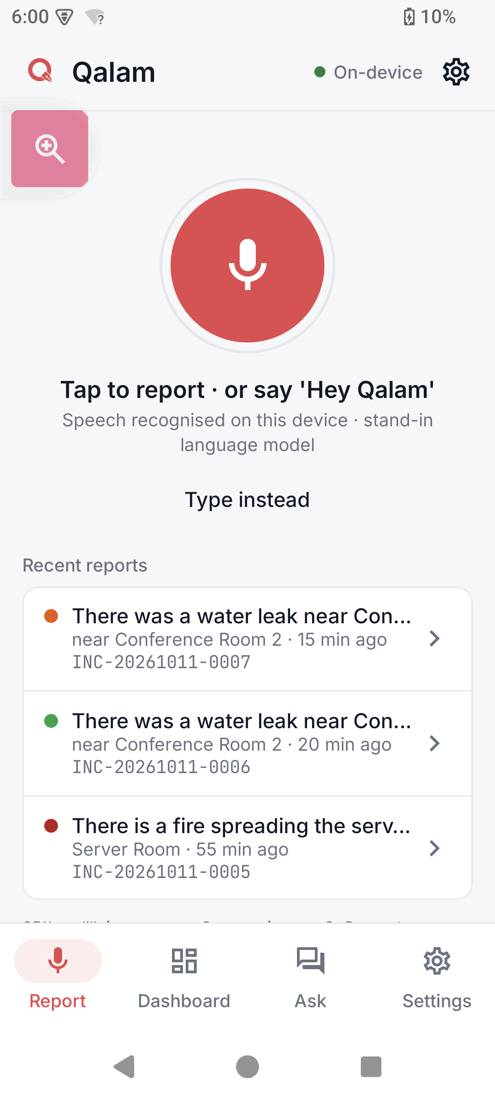
\includegraphics[height=6.1cm]{img/home.png}\hspace{3mm}
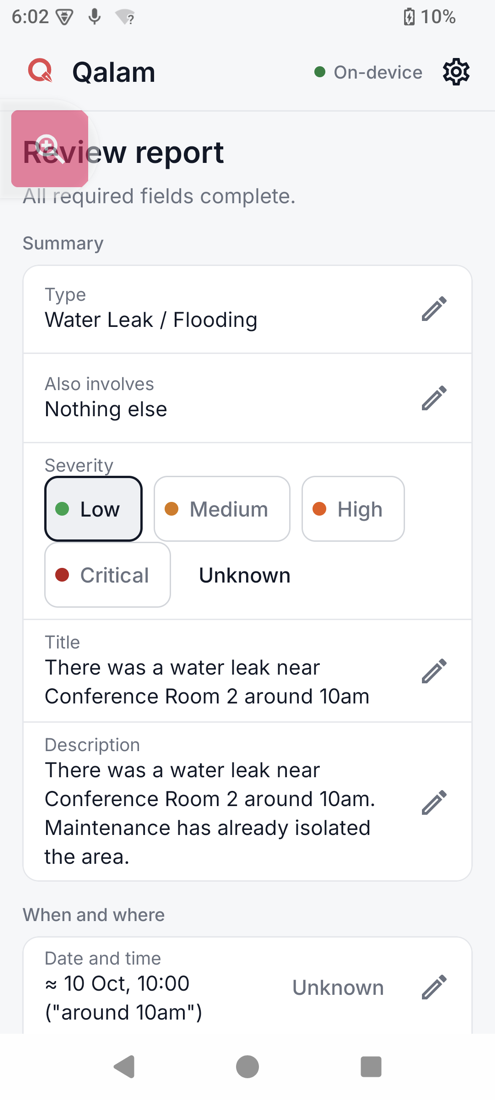
\includegraphics[height=6.1cm]{img/review.png}\hspace{3mm}
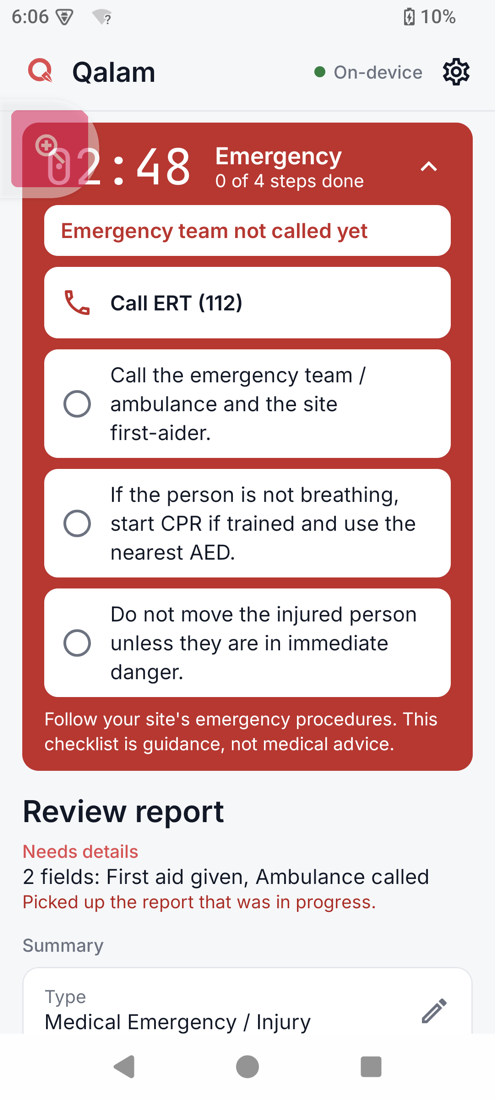
\includegraphics[height=6.1cm]{img/emergency.png}\hspace{3mm}
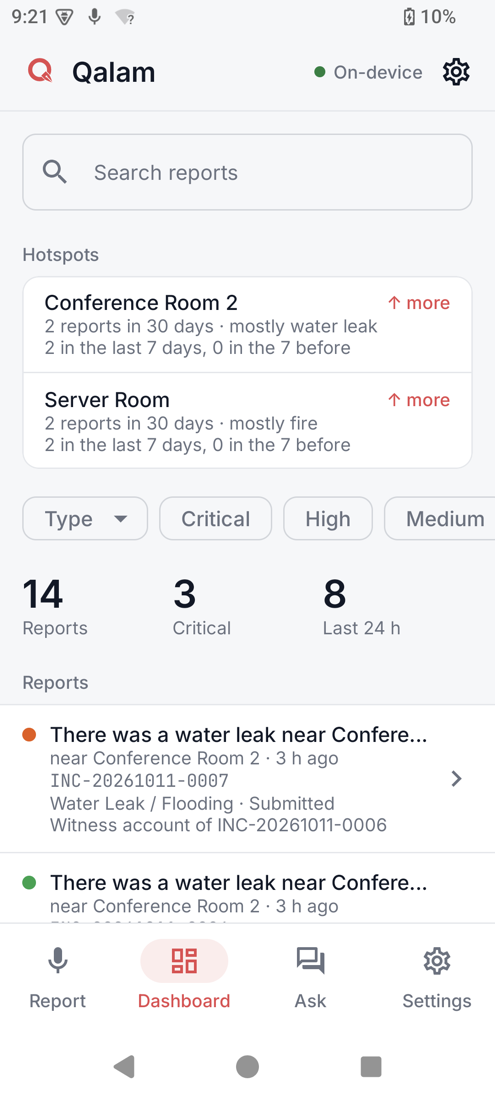
\includegraphics[height=6.1cm]{img/wow_dashboard.png}\hspace{3mm}
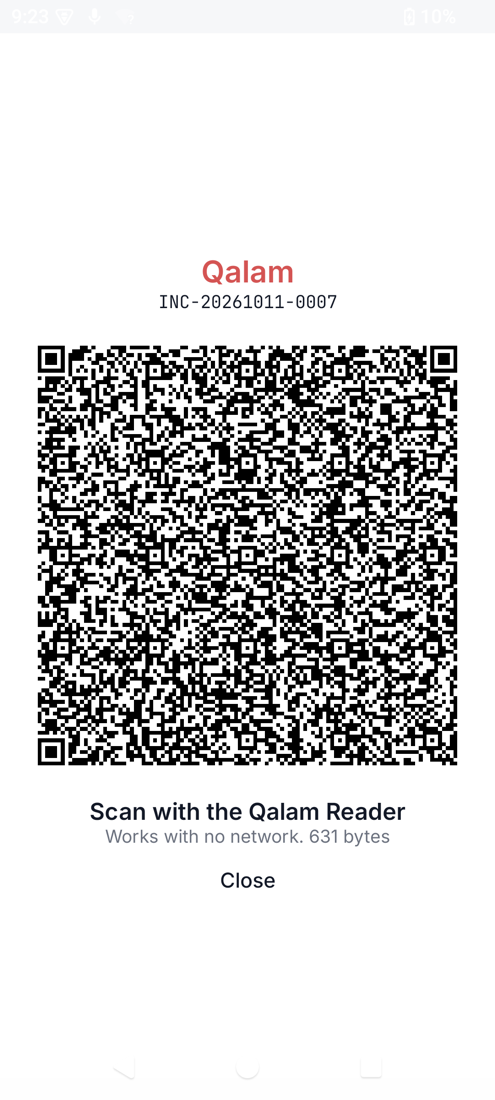
\includegraphics[height=6.1cm]{img/wow_qr.png}\\[2pt]
{\scriptsize Screenshots taken on the QIDK: home with the report button and proof line; review screen; emergency response clock; dashboard with hotspots; offline QR handoff.}
\end{center}

\section{Beyond the Brief}
\begin{tabularx}{\linewidth}{@{}p{3.1cm}L@{}}
\toprule
\textbf{Feature} & \textbf{What it does}\\
\midrule
Show your evidence & Tap any field on the review or detail screen and the transcript words that support it light up. Every value is traceable to what was said.\\
Response clock & Turns a report into action during an emergency: timer, SOP checklist, ``Call ERT'', a reminder if the team has not been called, and a response timeline stored with the report.\\
Hands-free start & Quick Settings tile, app shortcut, home-screen widget, and the wake phrase ``Hey Qalam'' (offline Vosk listener that hands the microphone to Whisper).\\
Multi-witness merging & A second report of the same event is detected (place, category, time) and offered as a witness account; never merged automatically. A field-by-witness table highlights conflicts and a supervisor picks the trusted value, recorded in the audit log.\\
Repeat incidents and hotspots & The dashboard flags places and hazards that keep recurring, with a 7-day trend, and marks a new report that repeats an earlier one.\\
Ask about reports & Typed or spoken questions over the local database (``what happened in Bay 4?'', ``how many critical this week?''), answered from structured filters plus semantic search.\\
Offline QR handoff & A report leaves the device with no network at all: the app shows one QR code (compressed, CRC-checked), and \emph{Qalam Reader}, a single self-contained web page, scans it and produces a one-page PDF.\\
Product design & One accent colour, lists instead of cards, Inter and JetBrains Mono bundled, label-above-value forms with ``Required'' and ``Check'' markers; readable on a projector.\\
\bottomrule
\end{tabularx}

\section{Results}
All numbers were measured on 11th October; the full tables, method and caveats are in \code{eval/RESULTS.md} and \code{eval/asr\_benchmark.md}.

\begin{tabularx}{\linewidth}{@{}p{4.4cm}L@{}}
\toprule
\textbf{Measurement} & \textbf{Result}\\
\midrule
LLM speed on the QIDK NPU & \textbf{22--23 tokens/s}; time to first token 0.5--0.7\,s with the full prompt; extraction \textbf{4.4\,s} median in the app, a follow-up answer \textbf{1.8\,s}; model load 3.4\,s.\\
Speech recognition & Whisper-small: WER 7.0\,\% measured on the board on our English clips; \textbf{2.8\,\%} with the domain hint (same model and settings, scored offline on 15 scripted clips); about 1.8\,s on the board for a 10\,s utterance. Against tiny.en (8.2\,\%) and base.en (4.9\,\%) with the same hint, small is the most accurate and still 5.6$\times$ faster than real time.\\
End of speech to filled form & About 8\,s, the target set in M1 (sum of the measured stages: recognition 1.5\,s, a 2\,s ``heard this'' pause the user can skip, extraction 4.4\,s).\\
Stability & 18 consecutive reports on the board without a restart: no crash, latency flat, 42--49\,$^\circ$C. Reports survive an app kill; an emergency in progress is picked up again.\\
Offline proof & No \code{INTERNET} permission in the APK; 0 bytes sent by the app (system counter shown in the app).\\
Automated tests & \textbf{440 passing} (validator, parser, normalisers, state machine, merge and hotspot rules, QR codec, database on a real SQLite), plus the web reader's decode, image and headless-browser tests.\\
\bottomrule
\end{tabularx}

\pagebreak
\textbf{Extraction accuracy, system versus components.} Held-out split of our 150-case text set (108 cases, never used for the model prompt), run on the board through the app's own post-processing code:

\begin{center}
\begin{tabular}{@{}lccc@{}}
\toprule
 & \textbf{Rules only} & \textbf{Qwen3-4B raw} & \textbf{Qalam system}\\
\midrule
Incident-type accuracy & 95.4\,\% & 90.7\,\% & \textbf{95.4\,\%}\\
Field precision / recall / F1 & 0.92 / 0.57 / 0.71 & 0.60 / 0.39 / 0.47 & 0.73 / 0.41 / 0.53\\
Valid tool calls & 100\,\% & 95.4\,\% & 95.4\,\% (rest answered by rules)\\
Fields filled without evidence & 2.5\,\% & 28.8\,\% & 18.4\,\%\\
\bottomrule
\end{tabular}
\end{center}

How to read this. The system layer lifts the model from 90.7\,\% to 95.4\,\% on incident type and removes about a third of its unsupported fields. The rules baseline looks strong because it was tuned on these template sentences, so its figures are an upper bound; on Hinglish the system is already ahead of it (62 against 61 of 66). The remaining gap in recall is by design: the compact NPU prompt extracts the common fields and leaves category details to the follow-up questions, which is what the validator loop is for. Prompt work mattered: the first prompt scored 51.9\,\% on the same cases; the current one, which also receives a keyword hint from the rules, 90.7\,\%.

\textbf{Behaviour on the board (typed into the live app, NPU model):} water leak from the problem statement (asks only for injuries and leak source), Hinglish with ``aadha ghanta pehle'', small talk, the self-correction ``at 10, no, 11'', and ``there's a leak'' (asks for exactly the missing fields) all pass; 6 of 10 cases pass outright, 3 partly, 1 fails (a second incident in the same sentence is not split out yet).

\textbf{Speech-recognition model choice} (WER on 15 scripted English clips, same decoding; time for a 10\,s clip on the QIDK):

\begin{center}
\begin{tabular}{@{}lccc@{}}
\toprule
 & \textbf{tiny.en} & \textbf{base.en} & \textbf{small (shipped)}\\
\midrule
WER without / with the domain hint & 10.3\,\% / 8.2\,\% & 6.8\,\% / 4.9\,\% & 4.4\,\% / \textbf{2.8\,\%}\\
WER on 9 noisy live recordings, without / with hint & 27.9\,\% / 10.5\,\% & 14.0\,\% / 5.8\,\% & 9.3\,\% / 2.3\,\%\\
Time on the QIDK & 0.25\,s & 0.41\,s & 1.8\,s\\
\bottomrule
\end{tabular}
\end{center}

\section{How We Tested}
\begin{itemize}
\item \textbf{Text set:} 150 template-generated cases over all categories (complete reports, missing fields, self-corrections, filler words, relative times, Hinglish), each with the expected value of every field; a dev split of 42 was fixed before prompt work and results are reported on the 108 held-out cases.
\item \textbf{Three columns, one harness:} rules only, the raw model, and the whole system. The system column is produced by the app's own Kotlin post-processing called from a JVM harness, so what is scored is what the user would see in the form.
\item \textbf{On the device:} every model output in the tables was generated on the QIDK's NPU. Ten behaviour cases and an 18-report soak run were driven through the installed app; speech recognition was timed on the board for three Whisper models.
\item \textbf{Scoring:} enums exact after normalisation, location against the site registry, time within $\pm$15 minutes, description scored separately; valid tool-call rate and the rate of fields filled without evidence are reported next to accuracy.
\item \textbf{Automated:} 440 unit tests run on every merge to \code{main}; the QR code shown on the board was decoded with the web reader's own code and passed its integrity check.
\end{itemize}

\section{Changes since M2, Limitations and Next Steps}
\begin{itemize}
\item \textbf{Model change.} The Llama 3.2 3B export did not finish in time, so we moved to Qualcomm's pre-compiled Qwen3-4B bundle for the same chip. Because the engine interface and prompt builder are model-agnostic, the switch took a chat template, one packaged library and a compact prompt.
\item \textbf{Two engine issues found and handled.} In-app loading needed \code{libQnnHtpNetRunExtensions.so} in the APK; and this bundle's Genie session fails after any prompt above about 500 tokens, so the app re-creates the session in the background after each call (3.4\,s, while the question is being spoken).
\item \textbf{Honest limits.} Spoken Hinglish is transcribed in English mode and is the weakest path (typed Hinglish gets Hinglish questions). Field recall of the model is below the rules baseline on the templated set. The wake phrase uses sound-alike words and was measured on a small sample only. Free-form test sentences written by people and the recorded-clip end-to-end run were not completed.
\item \textbf{Next.} A base-versus-fine-tuned comparison of the language model, Whisper on the NPU, a signed QR payload, and splitting two incidents spoken in one sentence.
\end{itemize}
\end{document}
